\documentclass{article}
\newcommand{\DOCTITLE}{}
\newcommand{\MODULE}{Robotics Lab}
\newcommand{\PROF}{Prof.\ Dr.\ Björn\ Hein}
\newcommand{\SEMESTER}{SS\ 25}

\newcommand{\header}{
  \begin{center}
    \Large\textbf{\DOCTITLE\ \\ \MODULE\ \\ \PROF\ \\ \SEMESTER}
  \end{center}
}

\newcommand{\makeHeader}{\header}
\usepackage{microtype}
\usepackage{mathtools}
\usepackage{amsfonts}
\usepackage{href-ul}
\usepackage{color,soul}
\begin{document}
    \pagenumbering{gobble} % Suppress page numbers on title and TOC pages
    \makeHeader\newpage
    \tableofcontents
    \newpage
    \pagenumbering{arabic} % Start page numbering from here
    \section{Set-up and operating instructions}
        The dispenser needs to be positioned so that the front of the dispenser is facing outside the front of the KUKA box. It needs to be positioned precisely so that the front clamp can be positioned at B9 and the back clamp can be positioned at B13. This is relevant since picking the blocks from the dispenser uses measured positions.
        
        The playing field can be positioned anywhere the robot can reach all cells on the field. Our test runs have been mainly using the points G3 and O3 as ankers. Should the field be moved to another position please keep in mind to adjust the taught base, \#17 by retraining the base with the three point method. 

        For the robots procedural setup of the game the user will have to continuously refill the dispenser by hand. This is because the player storage areas hold twelve blocks each, the dispenser only seven at maximum. First the storage of player 1 is filled with all 12 blocks, the storage of player 2 will be filled accordingly.

        Once the game is set up the user will be asked to choose a gravity mode out of the options of `gravity on' and `gravity off'. Gravity on will mean that both players will only be able to pick the bottom most cell of each column that is not already occupied by a piece. Gravity off will mean that both players can pick any unoccupied cell on the entire game area.

        The user will now be asked to pick a gamemode out of the options `PvP' (player vs player), `PvR' (player vs robot) and `RvR' (robot vs robot). In case PvR is played, the starting player has to be chosen as well.

        
        PvP\@: Two external players play against each other using the robot interface, which will ask for a move input at the start of each turn. 
        
        PvR\@: One player will be external, the other player will be played by the machine. At start of each of the external players turns the interface will ask for move input and subesequently make it's own prefered move.
        
        RvR\@: The robot will play against itself. The interface will not ask for any input and the game will run until one of the players has won or the game has ended in a draw.

        Finally, once either player has won or the turn count has reached 24 turns the game will end and in infomessage will be shown which the user will have to confirm. Upon confirmation the robot will clean up the game are by picking up the blocks from the game area and placing them back into the player storage. The dispenser will remain empty.
        The game can be reset by turning switch 1 to the right. After the current move is completed, the cleanup process will be started and the programm will terminate. Restarting the game without restarting the programm is not possible.

        At the start of each turn the interface will ask for a move input. This happens by the user first being prompted to select a column between 1 and 6 and then if gravity is off, a row between A and D. If gravity is on the prompt for the row will be skipped and the robot will automatically place the block in the lowest unoccupied cell of the selected column.
        \newpage

    \section{Program structure}
        \subsection{calc\_block\_placement.src}
            The \texttt{calc\_block\_placement.src} file contains the logic for determining the correct row position for a block to be placed in the Connect Three playing field, specifically when gravity mode is enabled. The main function, \texttt{calc\_block\_placement}, examines the selected column and iterates from the bottom row upwards to find the first available cell (marked as \texttt{\#free}). When such a cell is found, it sets the row coordinate in \texttt{next\_field.y} and returns, ensuring that blocks always `fall' to the lowest unoccupied position in the column. This file encapsulates the gravity placement rule and is called whenever a move is made in gravity mode.

            See Figure~\ref{fig:calc_block_placement}.

        \subsection{calc\_positions.src}
            The \texttt{calc\_positions.src} file is responsible for calculating and assigning the physical coordinates for all relevant positions in the Connect Three robot setup. The main function, \texttt{calc\_positions}, computes the locations for Player 1 and Player 2 storage spots as well as the positions of the game field cells. It uses step sizes and offsets to generate arrays of coordinates for each area, ensuring proper spacing and orientation. The function first calculates the storage positions for both players, taking into account the offset between their areas, and then determines the positions for each cell on the playing field based on a reference point (\texttt{PFA1}). This file is essential for mapping logical game positions to real-world robot coordinates, enabling accurate block placement and retrieval during gameplay.

            See Figure~\ref{fig:calc_positions}.

        \subsection{check\_game\_over.src}
            The \texttt{check\_game\_over.src} file implements the win detection logic for the Connect Three game. The main function, \texttt{check\_game\_over}, scans the playing grid for any sequence of three identical, non-free player markers in a row, column, or diagonal. It checks all possible horizontal, vertical, and both diagonal triplets. If a winning triplet is found, the function sets the \texttt{result} variable to the winning player and returns immediately. If no winner is found, \texttt{result} remains set to \texttt{\#free}. This file is essential for determining when the game has ended and which player, if any, has won.

            See Figure~\ref{fig:check_game_over}.

        \subsection{cleanup.src}
            The \texttt{cleanup.src} file automates the process of clearing the playing field at the end of a Connect Three game. The main function, \texttt{cleanup}, iterates over all cells in the playing field and identifies blocks belonging to Player 1 or Player 2. For each block found, the robot picks it up from its current position and places it back into the appropriate player’s storage area, incrementing the storage index as it goes. Cells marked as \texttt{\#free} are ignored. This file ensures that the game area is reset and all blocks are returned to storage, preparing the system for the next game or shutdown.

            See Figure~\ref{fig:cleanup}.

        \subsection{drai\_gaewint.src}
            The \texttt{drai\_gaewint.src} file is the main control program for a full Connect Three game session using the robot. It orchestrates the entire game flow, from initial setup to cleanup, and integrates user interaction, robot actions, and game logic.

            At the start, the program declares and initializes all necessary variables and arrays, including storage positions for both players and the game field grid. It then calculates the physical positions for all relevant areas using \texttt{calc\_positions}, moves the robot to its home position, and sets up the blocks in the storage areas.

            The user interface is invoked to select gravity and game mode via \texttt{ui\_helper}. Depending on the selected mode, the program configures the player types (human or AI) and randomly assigns the starting player in PvR mode using the \texttt{RandomInt} helper function.

            The main game loop manages player turns, move selection, and block placement. For human players, the UI prompts for input and validates moves; for AI players, the best move is calculated automatically. The program enforces gravity rules and ensures blocks are placed in valid positions. After each move, the robot picks a block from the correct storage area and places it on the field.

            After each turn, the program checks for a win or draw using \texttt{check\_game\_over}. If a player wins or the turn count reaches 24, the game ends. The victory dialog is shown via \texttt{ui\_helper}, and the robot performs cleanup by returning all blocks from the field to the appropriate storage areas.

            Overall, \texttt{drai\_gaewint.src} coordinates all aspects of the Connect Three game\@: setup, player management, move logic, robot control, win detection, user interaction, and cleanup, ensuring a complete and automated game experience.

            See Figure~\ref{fig:drai_gaewint}.

        \subsection{get\_best\_move.src}
            The \texttt{get\_best\_move.src} file implements the AI logic for selecting moves in Connect Three, along with supporting functions for board analysis and move generation. The main function, \texttt{get\_best\_move}, receives the current board state, the player for whom the move is being calculated, and outputs the best move coordinates.

            The AI begins by handling special cases for the first few turns, using hardcoded strategies to optimize opening moves depending on gravity and board state. For subsequent turns, it simulates all possible moves by iterating over playable cells, which are determined by the \texttt{get\_available\_moves} function. For each candidate move, the AI checks if it results in an immediate win, blocks an opponent's win, or improves its position. It uses a scoring system to prioritize moves: immediate wins are highest, blocking the opponent is next, and positional improvements are considered if no direct win or block is available.

            The supporting functions include:
            \begin{itemize}
                \item \texttt{get\_available\_moves}: Identifies which cells are playable, respecting gravity rules and ensuring only legal moves are considered.
                \item \texttt{copy\_board}: Copies the board state for simulation, allowing the AI to test hypothetical moves without altering the actual game state.
                \item \texttt{check\_win}: Checks if a given player has achieved a winning triplet (horizontal, vertical, or diagonal) on the board.
            \end{itemize}

            The AI logic is both offensive and defensive: it looks for moves that win the game, blocks the opponent from winning, and seeks to set up future opportunities. It also avoids moves that would immediately allow the opponent to win in the next turn. The combination of simulation, scoring, and rule-based heuristics makes the AI competitive and adaptable to different board states and game modes.

            See Figure~\ref{fig:get_best_move}.

        \subsection{pick\_from\_dispenser.src}
            The \texttt{pick\_from\_dispenser.src} file contains the robot motion sequence for picking up a block from the dispenser. The function begins by initializing the robot's movement parameters and enabling safety interrupts. It sets the appropriate base and tool data for the operation.

            The robot then moves through a series of predefined positions (XP1, XP2, XP5, XP4) using both point-to-point (PTP) and spline (SPTP) motions to approach the dispenser safely and accurately. At the correct position, the gripper is activated to close and grasp the block, with a short wait and error check to ensure successful gripping.

            After picking up the block, the robot moves away from the dispenser to a safe position, ready for the next operation. The sequence ensures collision-free, reliable block pickup, and integrates with the overall game flow for dispensing blocks to the playing field or storage. The file is essential for automating the interaction between the robot and the dispenser hardware.

        \subsection{pick\_from\_playingfield.src}
            The \texttt{pick\_from\_playingfield.src} file defines the robot sequence for picking up a block from a specified position on the playing field. The function receives a target coordinate and executes a series of precise movements to safely approach, grip, and lift the block.

            The robot first prepares the gripper and sets the appropriate base and tool data for field operations. It moves to a position above the target cell, then descends vertically to the exact location. The gripper is closed to grasp the block, and the robot then lifts the block back up to a safe height. Throughout the process, velocity and jerk parameters are set to ensure smooth and controlled motion.

            This file is essential for reliably retrieving blocks from the playing field, whether for cleanup, repositioning, or transferring to storage. It ensures that the robot interacts safely with the game area and minimizes the risk of collisions or dropped blocks.

        \subsection{place\_on\_playingfield.src}
            The \texttt{place\_on\_playingfield.src} file defines the robot sequence for placing a block onto a specified position on the playing field. The function receives a target coordinate and executes a series of controlled movements to safely approach, release, and withdraw from the placement location.

            The robot prepares the gripper and sets the correct base and tool data for field operations. It moves to a position above the target cell, descends vertically to the placement point, and then opens the gripper to release the block. After placement, the robot lifts back up to a safe height above the field. Velocity and jerk parameters are configured to ensure smooth and precise motion throughout the process.

            This file is essential for accurate and reliable block placement during gameplay, ensuring that the robot can interact with the game field without collisions or misplacement. It is used for both player moves and cleanup operations.

        \subsection{setup\_blocks.src}
            The \texttt{setup\_blocks.src} file automates the initial placement of blocks into the player storage areas at the start of the game. The function receives arrays of storage positions for both players and iterates through each position, picking a block from a generic storage location and placing it into the designated player storage spot.

            For both Player 1 and Player 2, the robot executes a loop that calls \texttt{pick\_from\_storage} to retrieve a block, then uses \texttt{place\_on\_playingfield} to deposit the block at the correct storage position. This ensures that all player storage areas are filled and ready for gameplay.

            The file is essential for preparing the game setup, guaranteeing that each player starts with the correct number of blocks in their respective storage areas. It streamlines the setup process and integrates with the overall game initialization sequence.

        \subsection{ui\_helper.src}
            The \texttt{ui\_helper.src} file provides all user interface dialogs and prompts for the robot program, allowing the operator to interact with the game setup and flow. The main function, \texttt{ui\_helper}, is called with a context argument (\texttt{ui\_caller}) and presents different dialog windows depending on the current phase of the game.

            In the \texttt{\#setup} case, the function prompts the user to select the gravity mode (on/off) and the game mode (PvP, PvR, RvR), storing the results in global variables for use in the main program. In the \texttt{\#place} case, it asks the user to select a column for placing a block, and if gravity is off, also prompts for a row. The selected coordinates are stored in \texttt{next\_field} for use in move execution.

            In the \texttt{\#victory} case, the function displays a message indicating the game result (draw, player 1 wins, or player 2 wins) based on the value of \texttt{active\_player}, and waits for user confirmation before proceeding.

            Dialogs are implemented using KUKA's internal dialog functions (\texttt{SET\_KRLDLG}, \texttt{EXISTS\_KRLDLG}), with options and messages tailored to each game phase. The function structure ensures that user input is collected, validated, and stored for use in the robot's game logic. This file is essential for all user interactions required during the game, from initial setup to move selection and end-of-game confirmation.

    \newpage
    \section{Suggestions for further development}
        The major pain point of the current implementation is that the robot is unable to calculate certain movements towards specific positions on the playing field, although they are reachable by manual input. Because of this the robot is unable to move to Cell 3A because it attempts to move there by rotating axis 5 and 6 instead of 2 and 3 in order to reach the position. 

        Other than this the main thing we would do if we had more time is refactoring the code to  improve readability and remove redundancy. This would happen mainly by extracting many sub functionalities to external functions within the same module, like in the drai\_gaewint.src file. 

        We also defined a new tool since the original tool was not centered correctly around the center of the gripper. This caused rotation around the z axis to be offset slightly. This problem could alternatively be fixed by training two seperate base coordinate systems, one for the game area and one for the storage area.
        
        Lastly, we would like to implement all motions with splines, when we originally did this the robot was for some reason unable to porform some motions, like the one to place a block down on a cell after already positioning above it. 

    \newpage
    \section{Flowcharts}
        \begin{figure}[htbp]
            \centering
            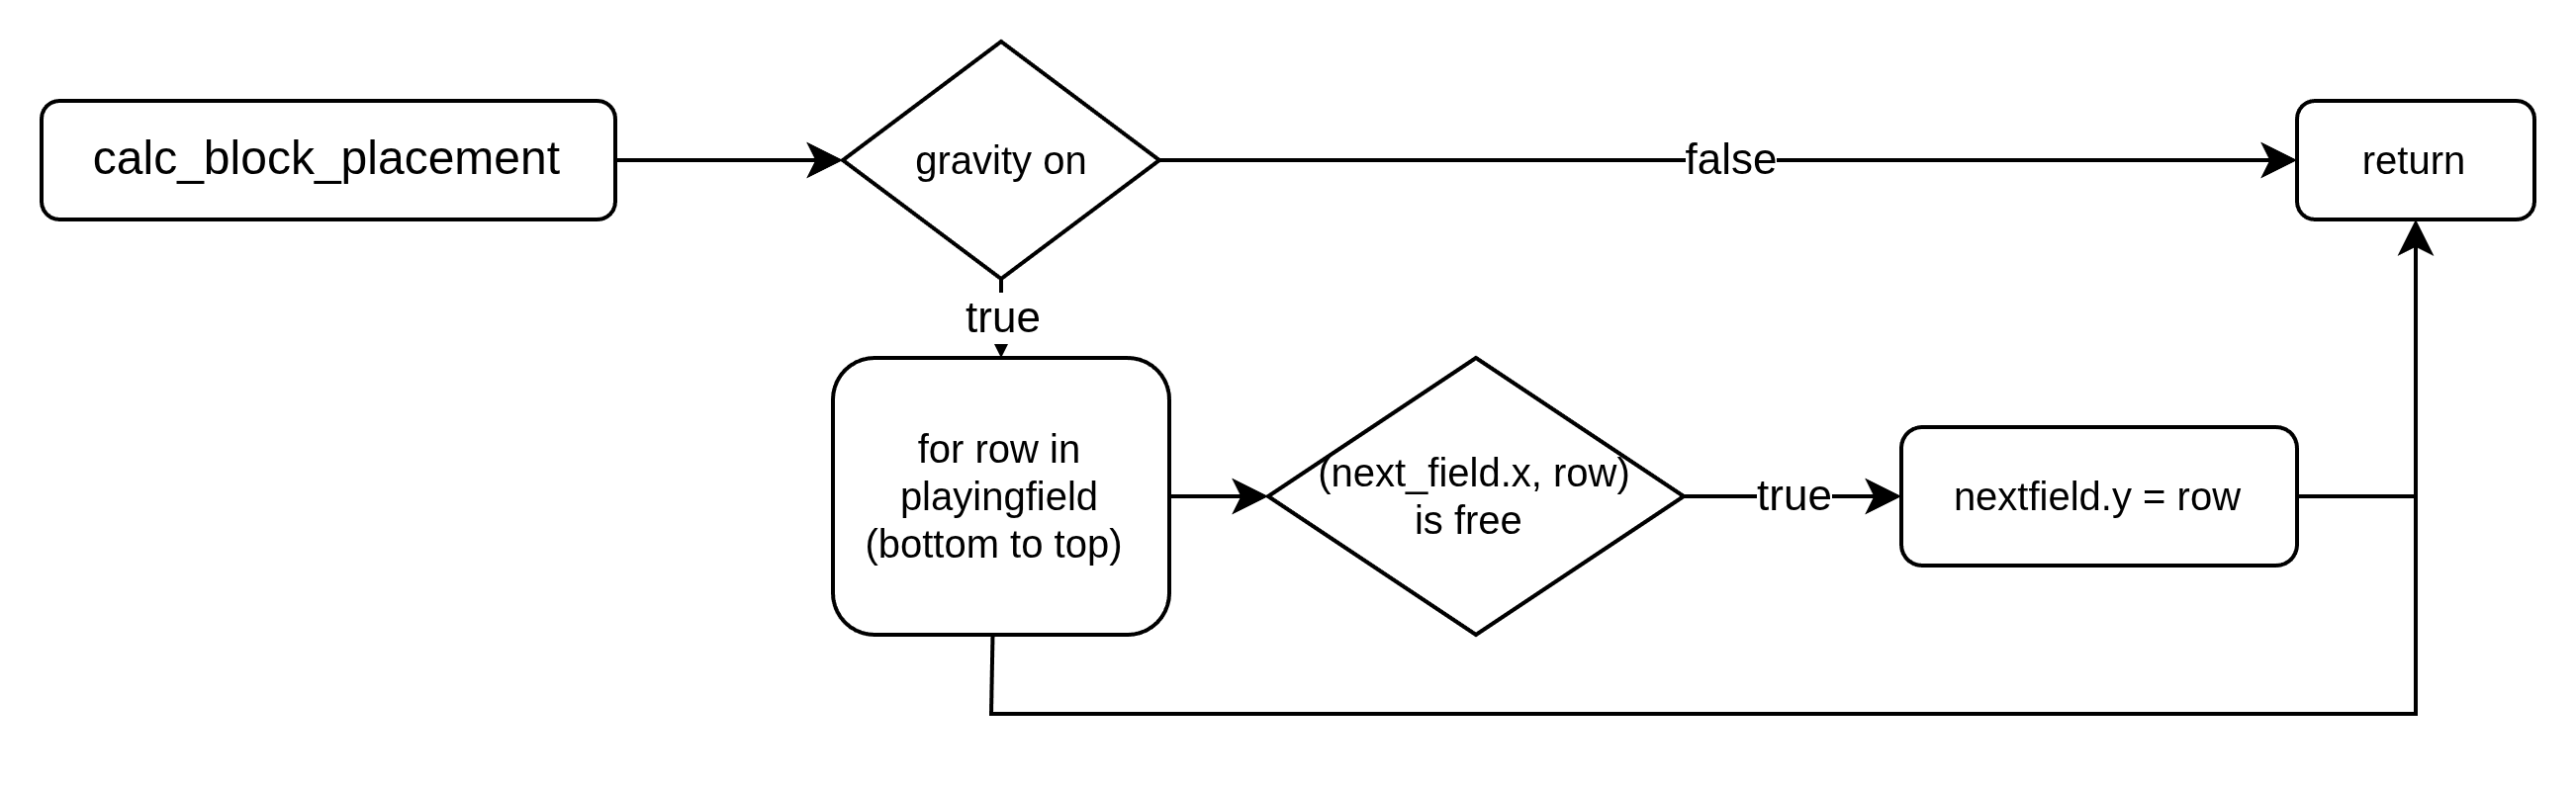
\includegraphics[width=\textwidth]{../media/calc_block_placement.png}
            \caption{Flowchart for \texttt{calc\_block\_placement} function}\label{fig:calc_block_placement}
        \end{figure}

        \begin{figure}[htbp]
            \centering
            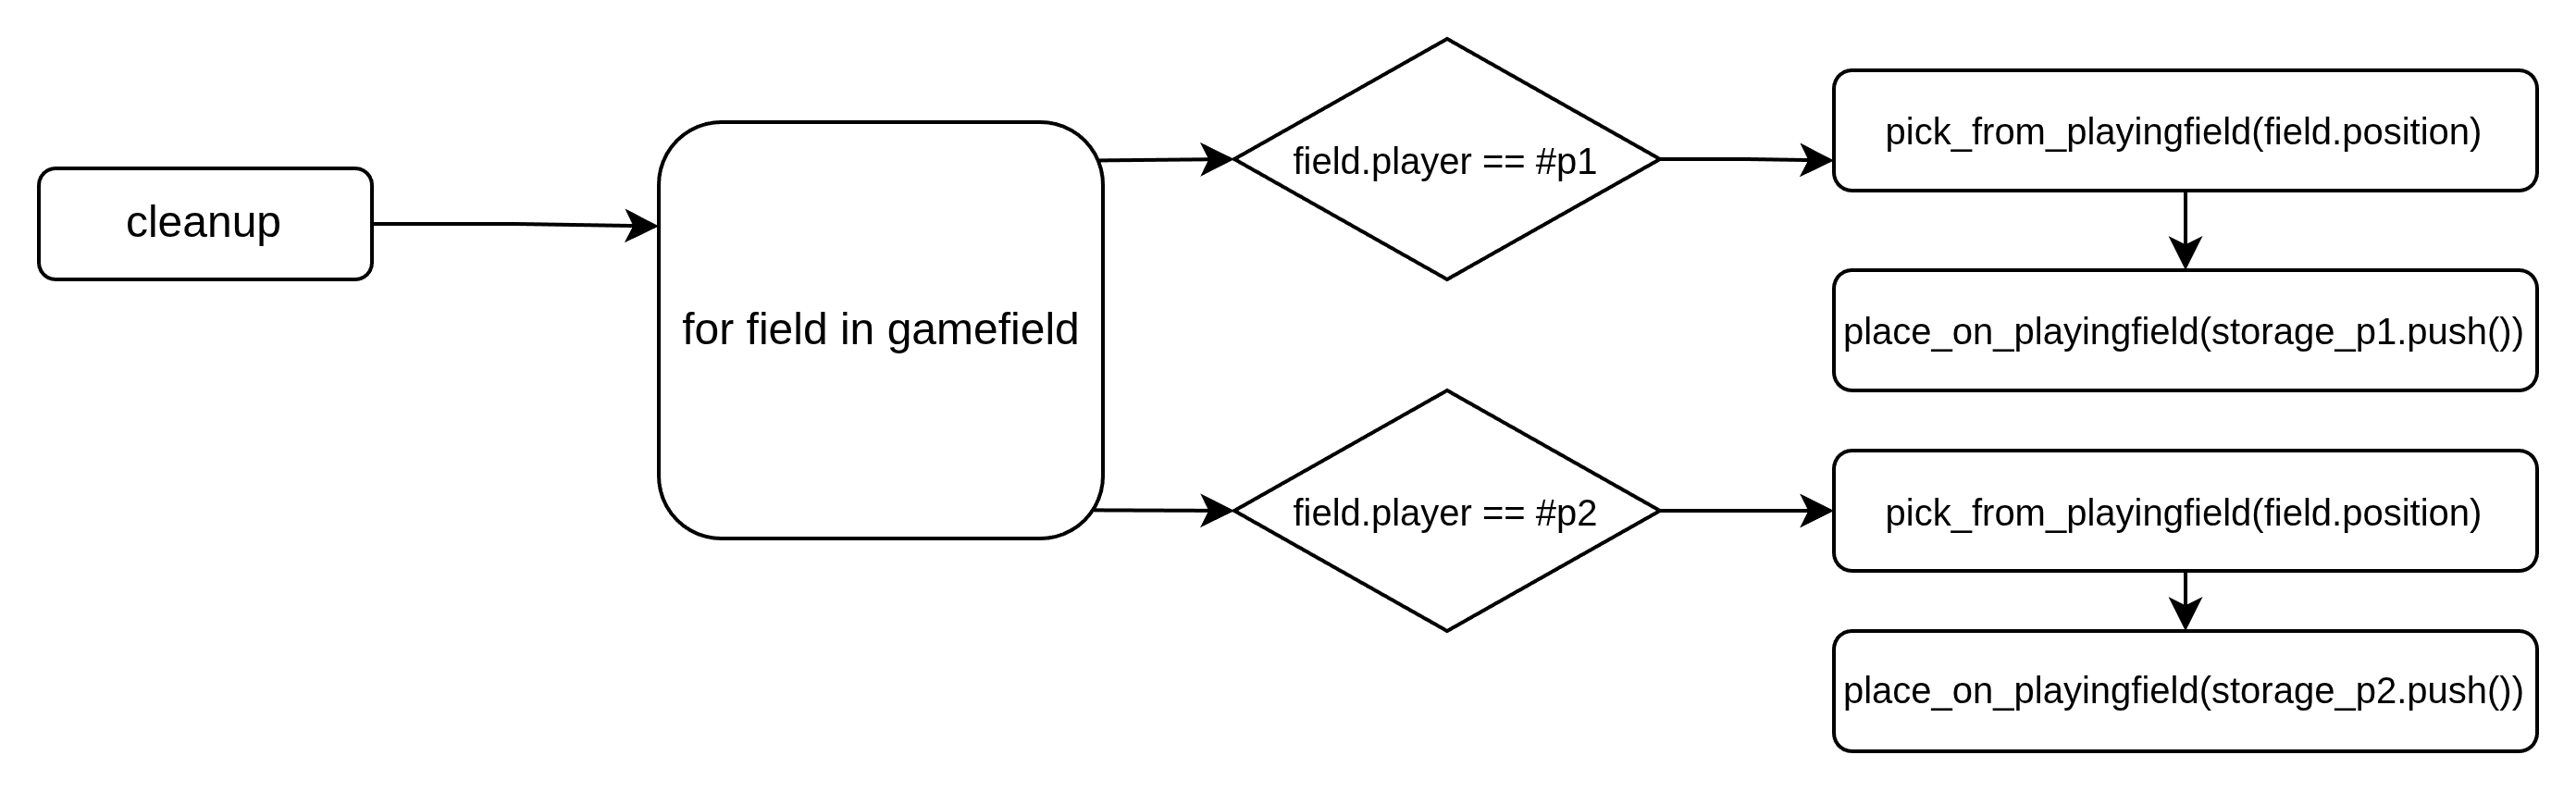
\includegraphics[width=\textwidth]{../media/cleanup.png}
            \caption{Flowchart for \texttt{cleanup} function}\label{fig:cleanup}
        \end{figure}

        \begin{figure}[htbp]
            \centering
            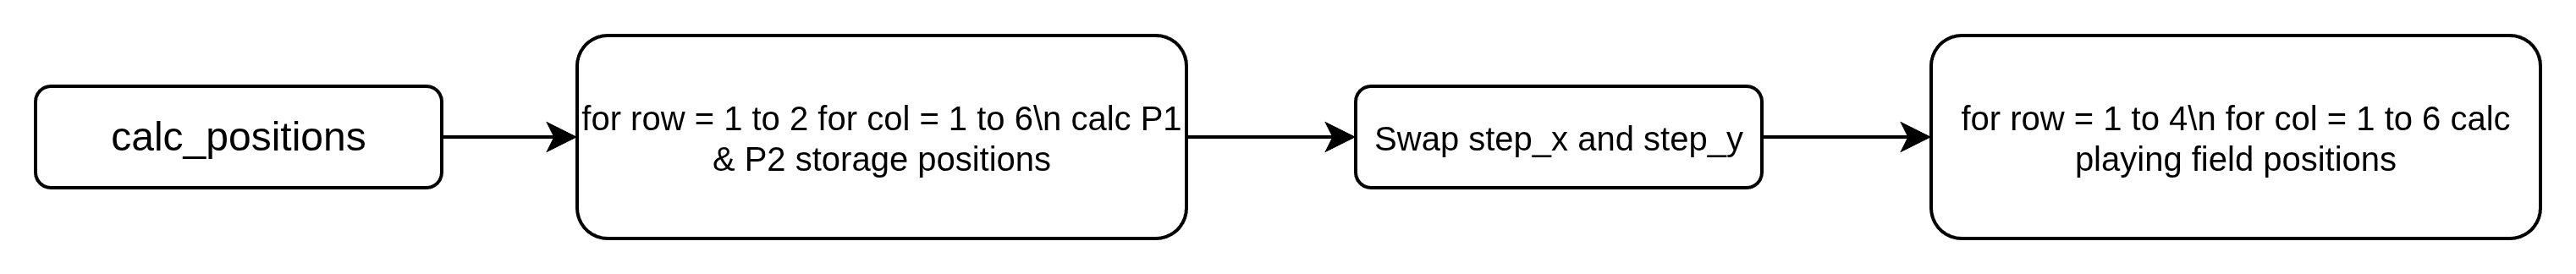
\includegraphics[width=\textwidth]{../media/calc_positions.png}
            \caption{Flowchart for \texttt{calc\_positions} function}\label{fig:calc_positions}
        \end{figure}

        \begin{figure}[htbp]
            \centering
            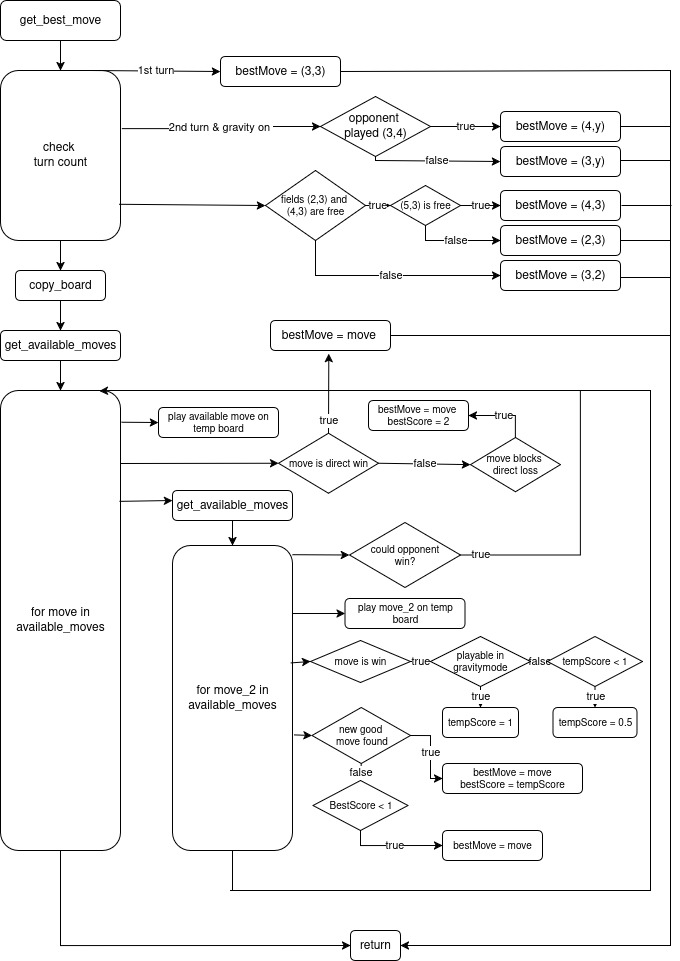
\includegraphics[width=\textwidth]{../media/get_best_move.jpeg}
            \caption{Flowchart for \texttt{get\_best\_move} function}\label{fig:get_best_move}
        \end{figure}

        \begin{figure}[htbp]
            \centering
            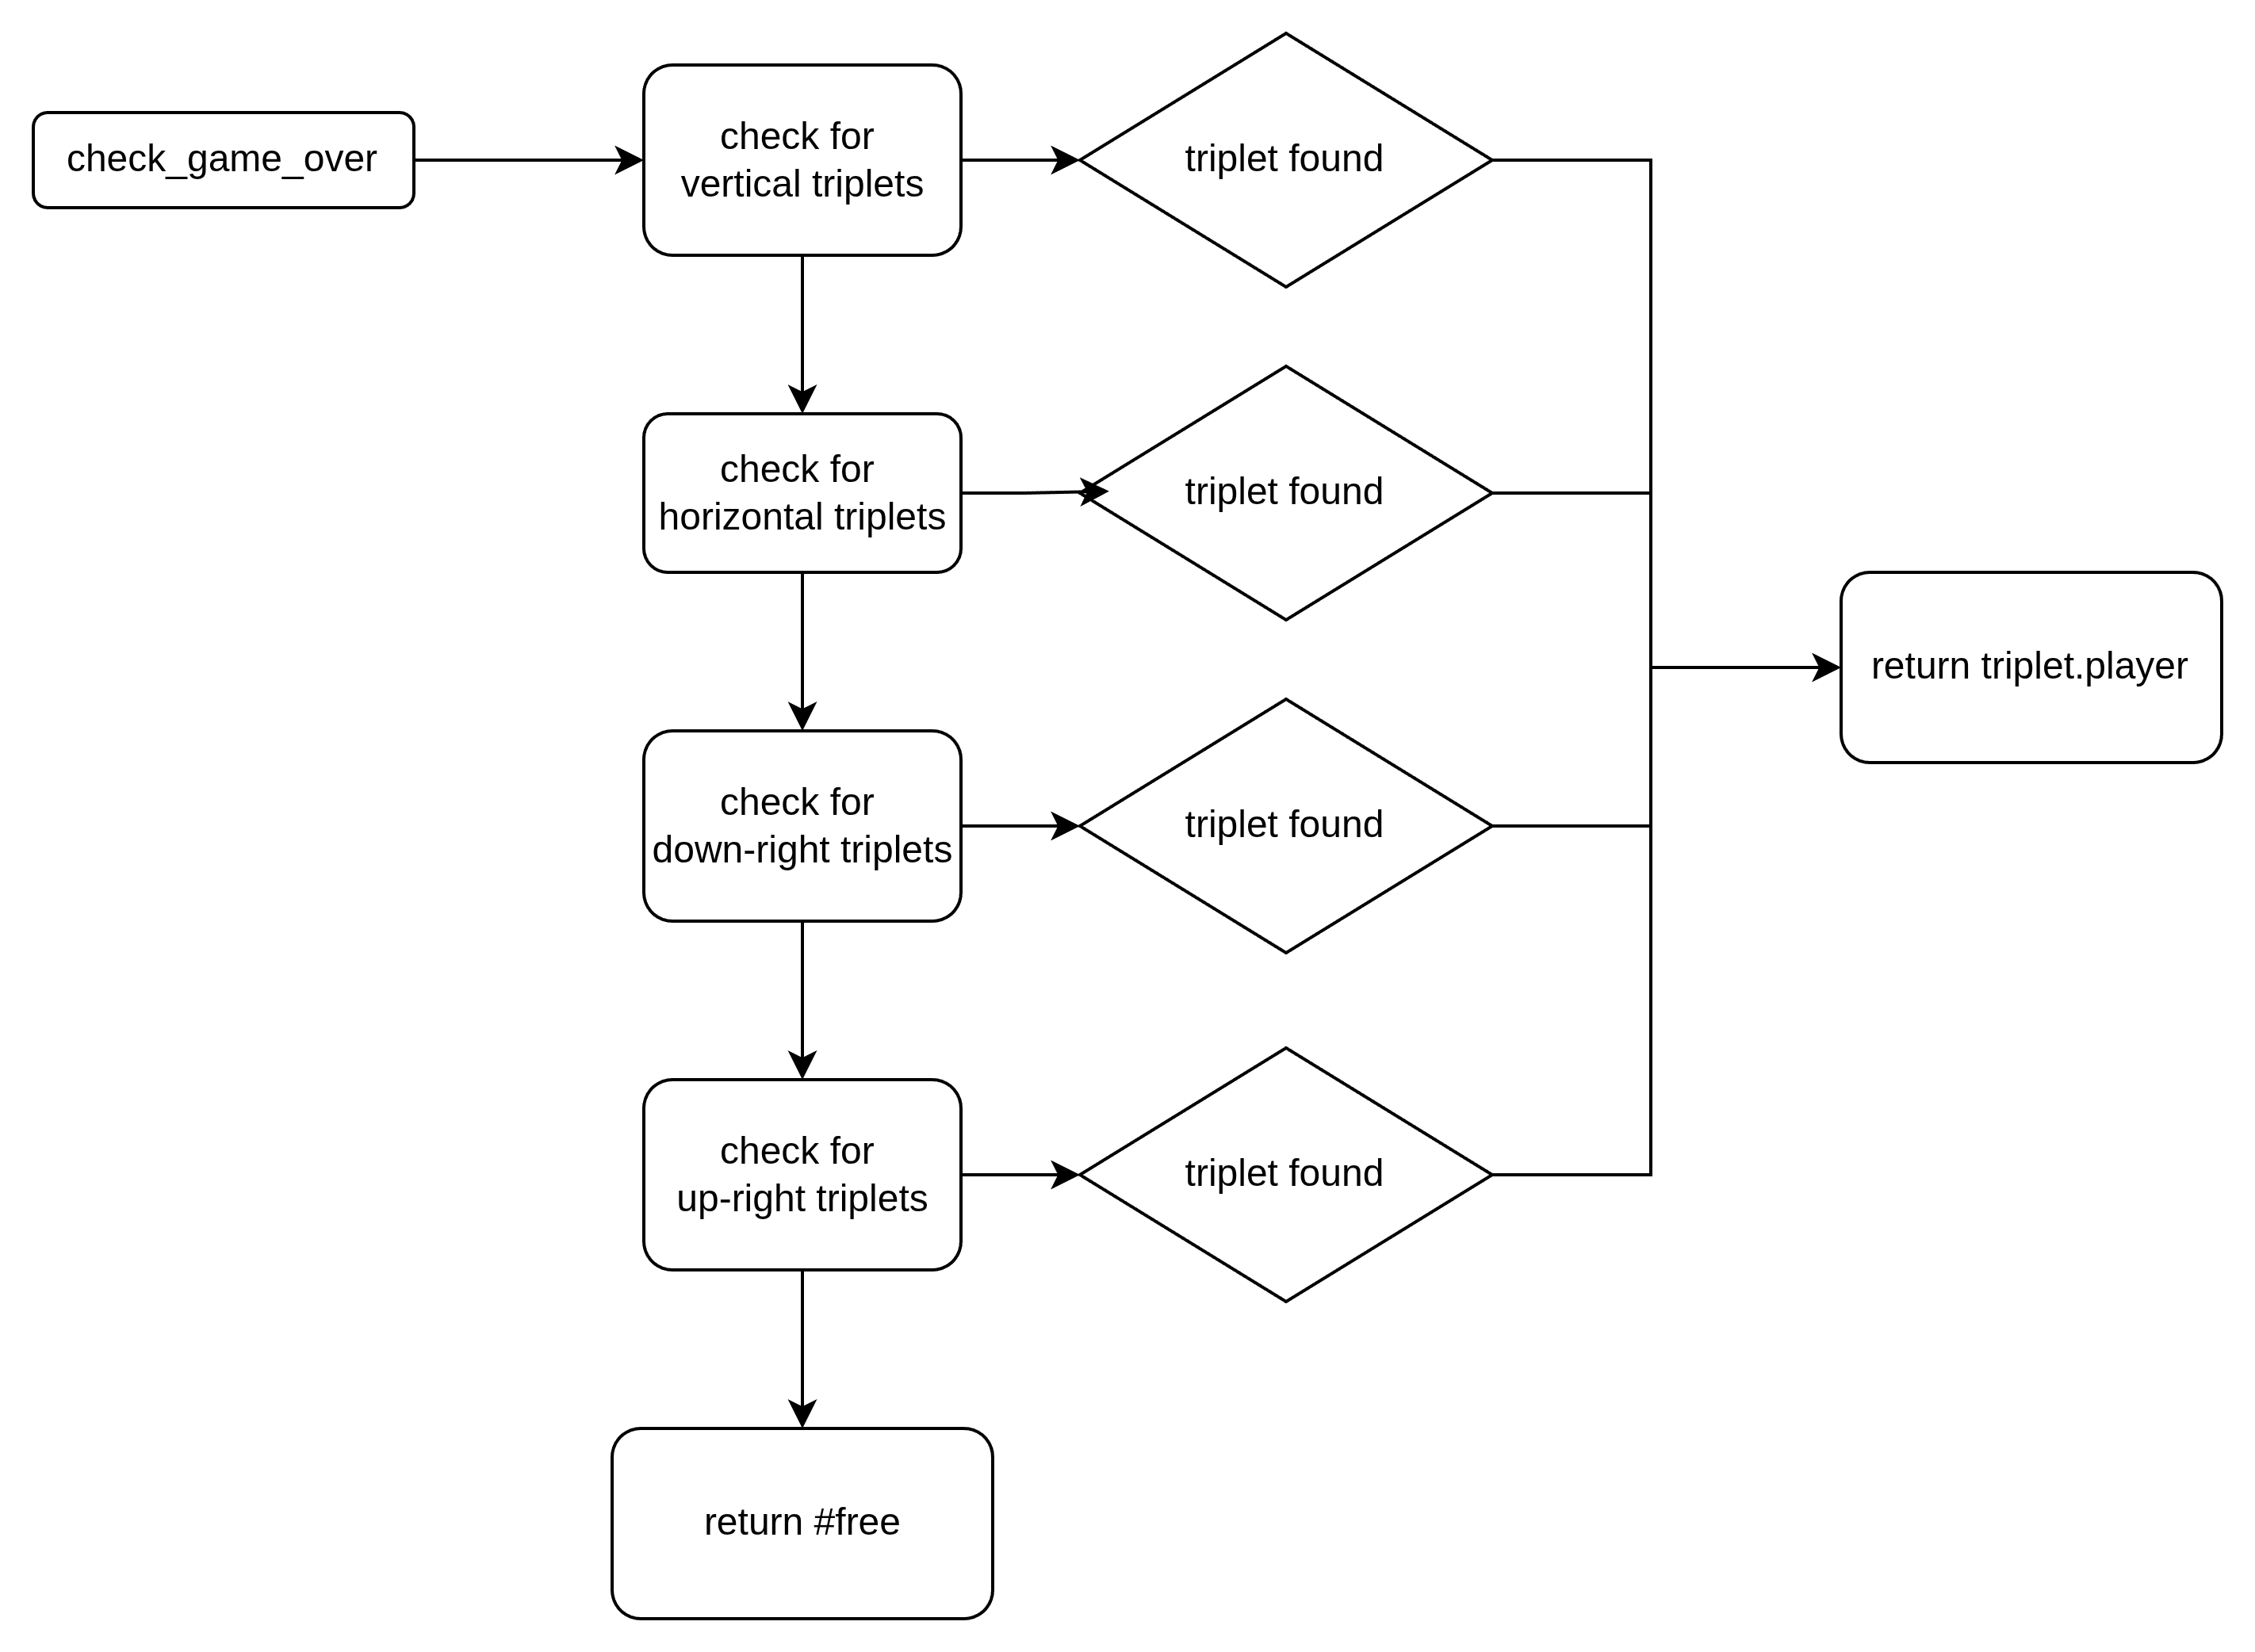
\includegraphics[width=\textwidth]{../media/check_game_over.png}
            \caption{Flowchart for \texttt{check\_game\_over} function}\label{fig:check_game_over}
        \end{figure}

        \begin{figure}[htbp]
            \centering
            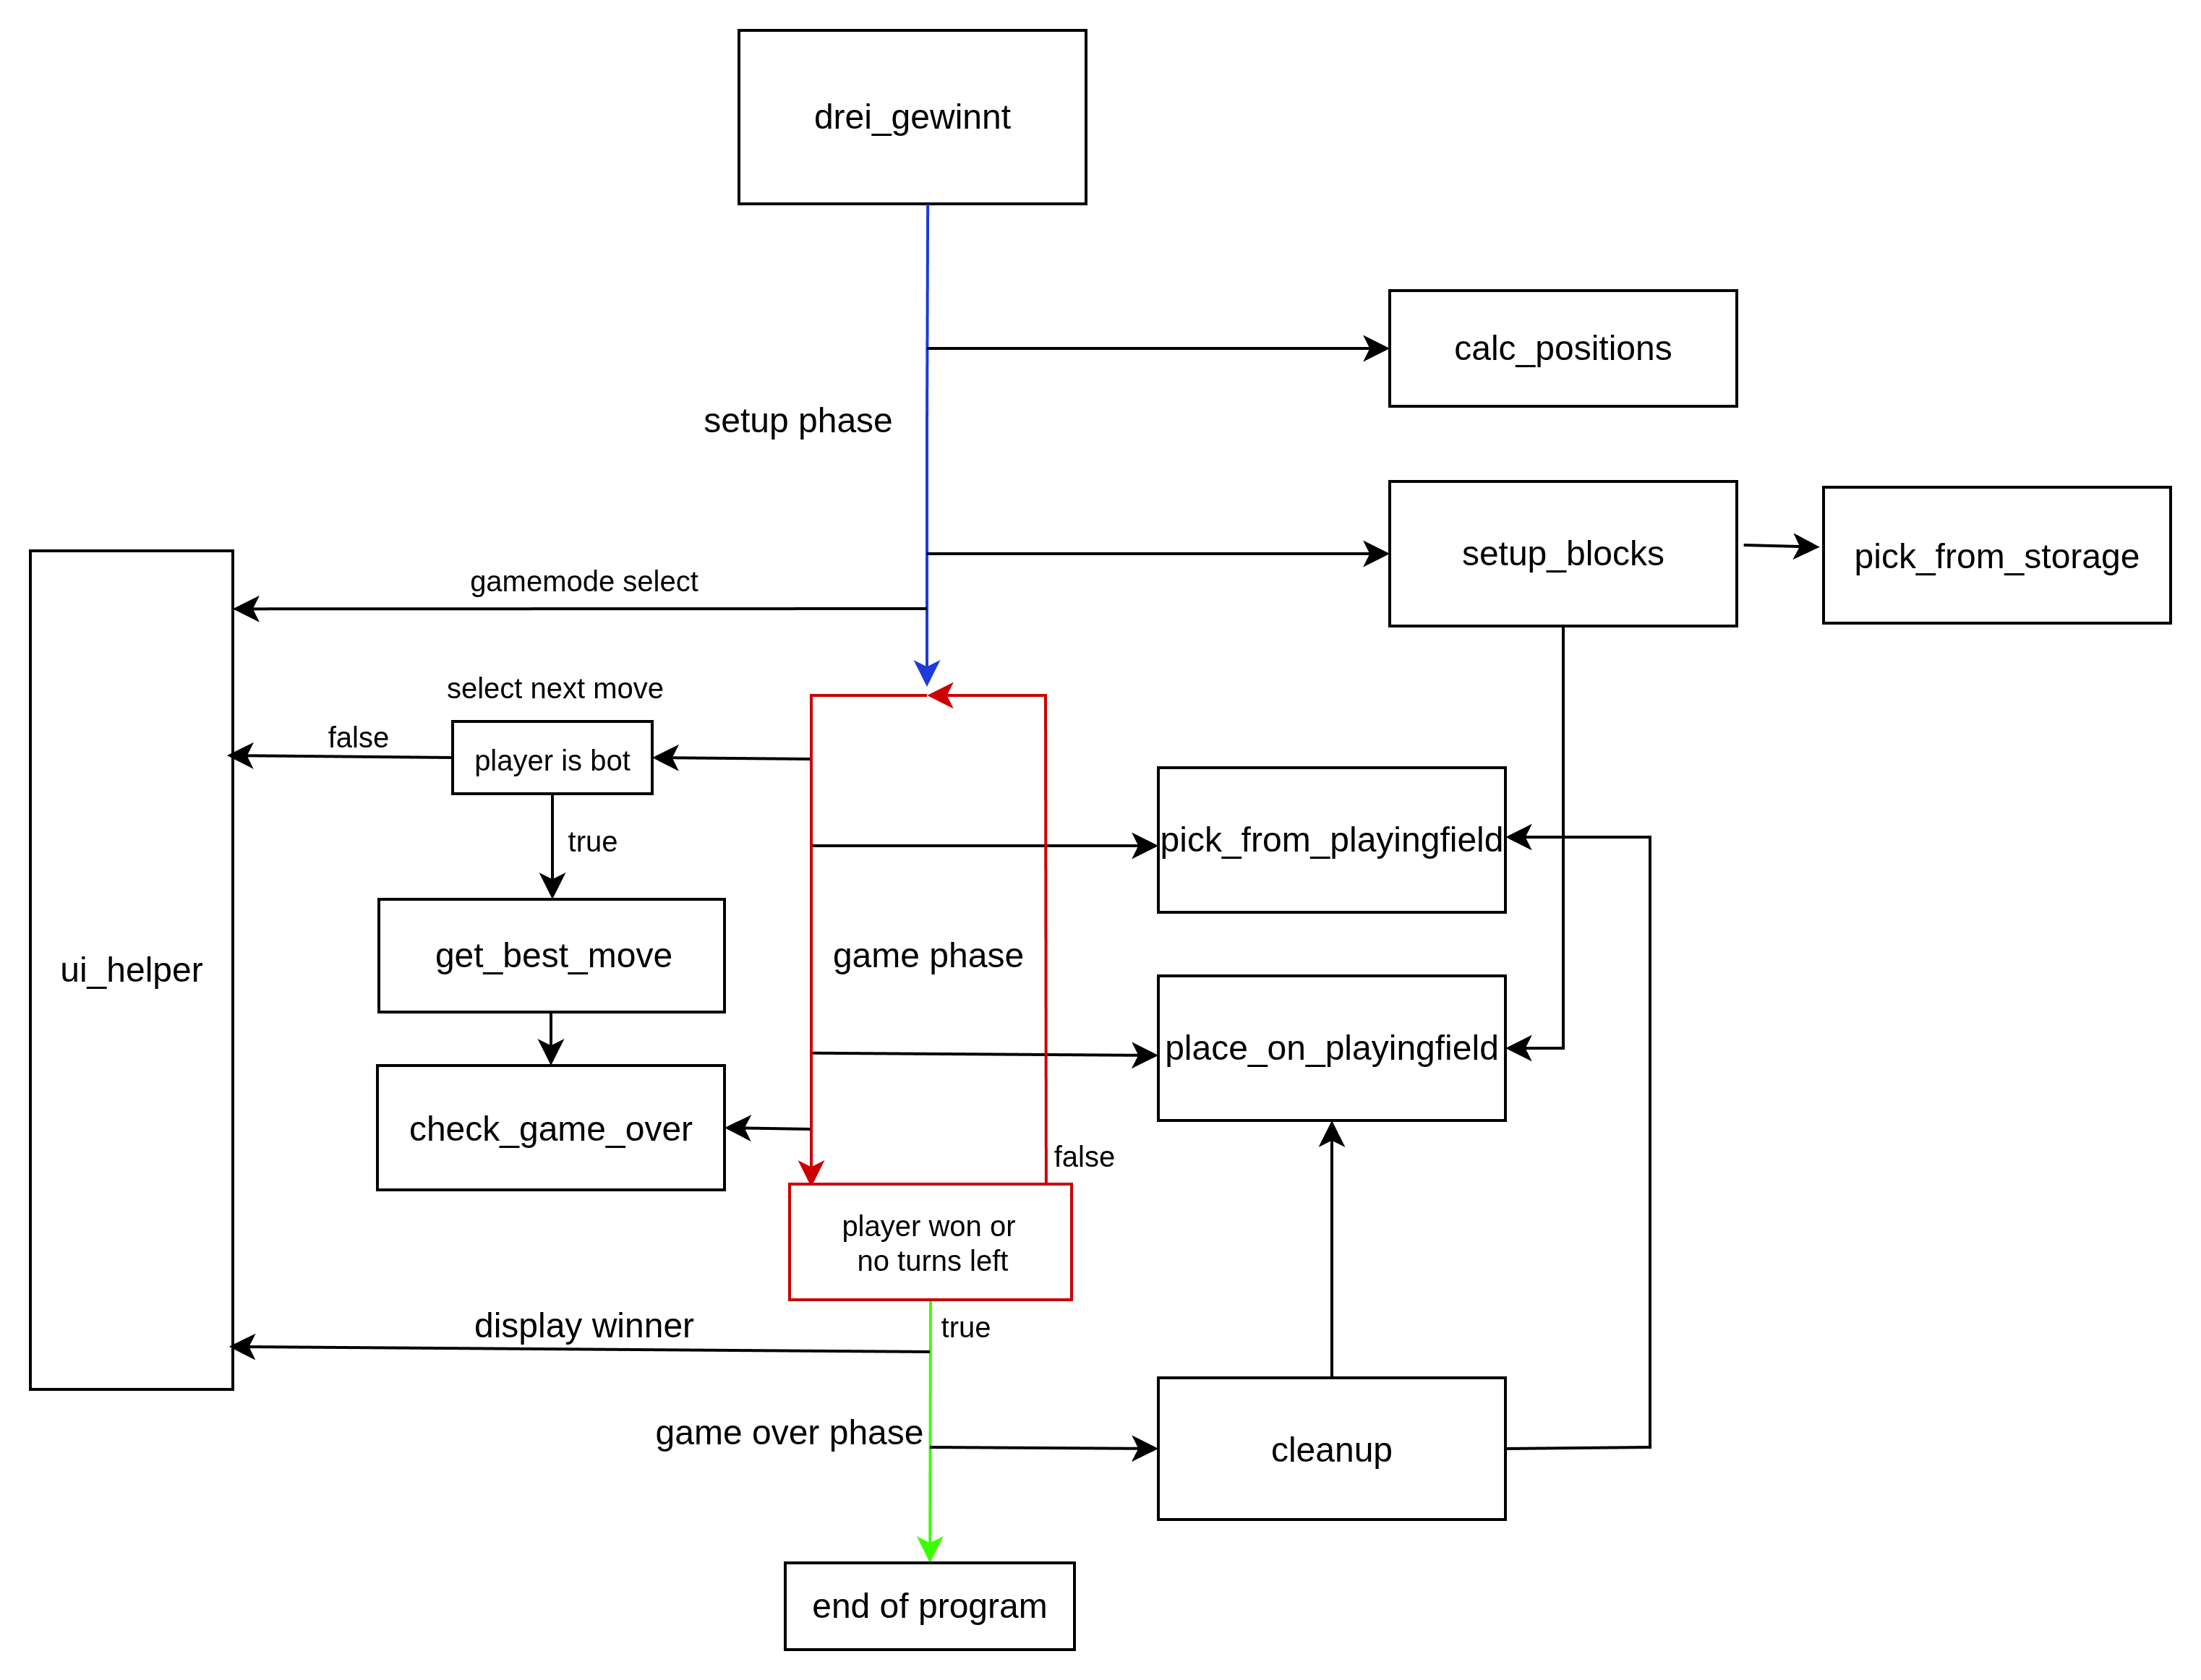
\includegraphics[width=\textwidth]{../media/drai_gaewint.png}
            \caption{Flowchart for \texttt{drai\_gaewint} function}\label{fig:drai_gaewint}
        \end{figure}

\end{document}